% Design & Architektur
% @author Tristan Ropers
%
\chapter{Design \& Architektur}

Zur Umsetzung der Anforderungen wurde eine RPC-Architektur entwickelt, die es ermöglicht den Prozess
abzubilden. Im folgenden Kapitel wird diese Architektur vorgestellt sowie ihre Besonderheiten.

\section{Systemkontext}

\begin{figure}[h]
 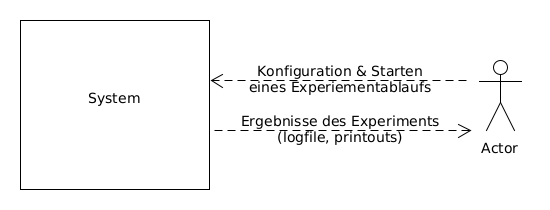
\includegraphics[width=\textwidth]{../diagrams/1_systemkontext.png}
 \caption{Systemkontext}
 \label{fig:systemkontext}
\end{figure}

Der Systemkontext des Gesamtsystems, wie in \ref{fig:systemkontext} zu sehen,
umfasst den Nutzer, welcher gleichzeitig Administrator ist und das Gesamtsystem.
Der Nutzer konfiguriert das System und startet im Anschluss die zuvor konfigurierte Konfiguration.
\clearpage

\section{Lösungsstrategie}

Das System besteht aus einer RPC-Architektur und einer Robotersimulation. Die RPC-Architektur ermöglicht
die Kommunikation und Steuerung der Abläufe der Roboter untereinander und dient damit als Basis der
Architektur. Alle Nodes laufen auf einem Rechner, laufen also jeder auf einem Port.
Um den Bereich abzustecken, in dem die Nodes laufen wird in der Konfiugration ein Portbereich mitgegeben.
Dieser Bereich dient auch der Kommunikation der Roboter. Über den Portbereich lassen sich Nachrichten
als Broadcast an jeden Port verschicken.

\subsection{Registrierung eines Roboters}

Die Roboter registrieren sich gegenseitig wenn das System hochgefahren wird. Sobald eine Node hochgefahren
wird, wird ein Broadcast auf dem Portbereich getätigt, damit wird jeder Roboter mit jedem bekanntgemacht
bevor die Wahl des Koordinators und Bestimmung des Zyklus losgeht. Somit hat man eine vollvermaschte
Peer-To-Peer Topologie.

\subsection{Bestimmung eines Zyklus}

Da die Nodes im System unabhängig von einer zentralen Einheit (bis auf Erhebung von Experimentdaten)
in einem Peer-To-Peer \citep{tanenbaumvansteen} Verbund existieren, muss zur Bestimmtung 
eines Zyklus eine Node die Rolle des Koordinators \citep{tanenbaumvansteen} übernehmen, welcher den Zyklus bestimmmt.\\
Zur Bestimmung des Koordinators wird zu Beginn des Experiments der Bully-Algorithmus \citep{tanenbaumvansteen}
als Wahlalgorithmus verwendet, bei diesem wird über die ID der Roboter bestimmt wer als
Koordinator gewählt wird.

\subsection{Schweißvorgang (Welding)}

Um den Schweißvorgang selbst zu simulieren wird beim welding() call in einer Node ein Thread gestartet,
der eine konfigurierte Zeit wartet um die mechanische Bewegung und das Schweißen der Roboter zu simulieren. Zusätzlich wird über die Konsole sowie in der Log-Datei eine Nachricht ausgegeben,
welche auf den Schweißvorgang hinweist.

\subsection{Logging der Prozessabläufe}

Um das Logging der verschiedenen Abläufe und Zustände sicherzustellen wurde ein Logging-Server implementiert,
der selbst über eine RPC Schnittstelle verfügt, auf dieser Log-Nachrichten der einzelnen Nodes übertragen
werden können.

\section{Architektur}

\subsection{Gesamtsystem}

\begin{figure}[h]
 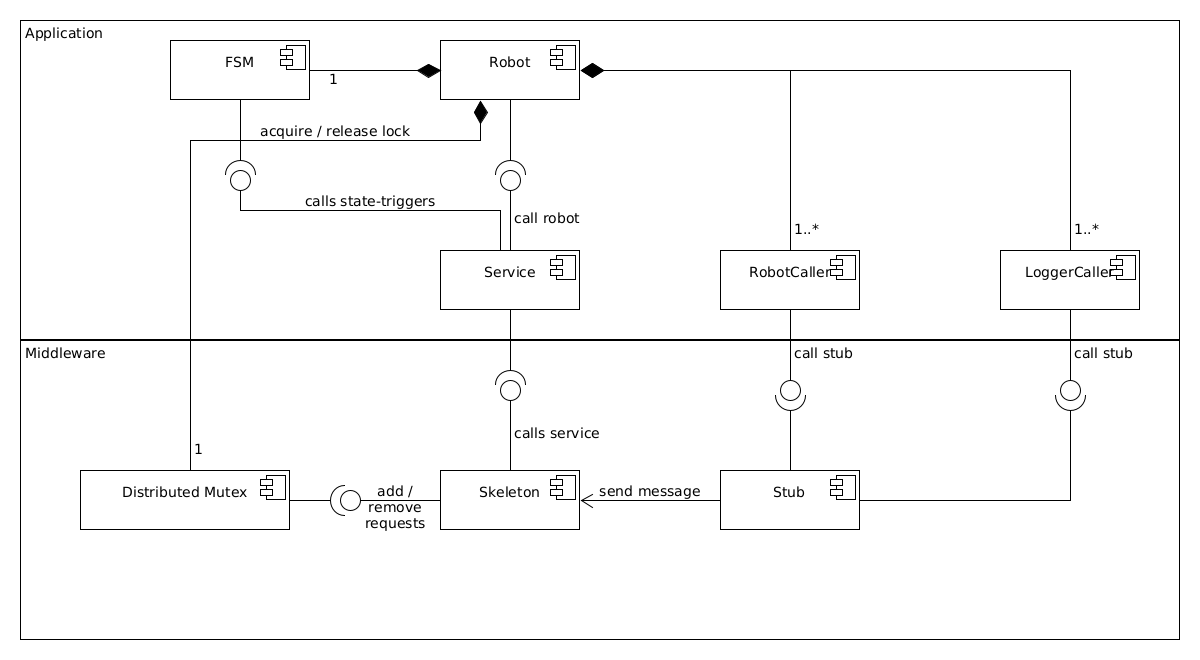
\includegraphics[width=\textwidth]{../diagrams/2_gesamtsystem.png}
 \caption{Komponentendiagramm Gesamtsystem}
 \label{fig:gesamtsystem}
\end{figure}

\subsection{Robot}

Eine zentrale Rolle in der Architektur spielt der Roboter, er beinhaltet Kommunikationselemente (Stubs 
\citep{tanenbaumvansteen} zu den anderen Robotern), eine Statemachine, eine Simulation des
Schweißvorgangs (siehe \ref{fig:gesamtsystem}) und eine Implementierung des verteilten gegenseitigen
Ausschluss (IDistributedMutex \ref{fig:gesamtsystem}).

\clearpage

\begin{figure}[h]
 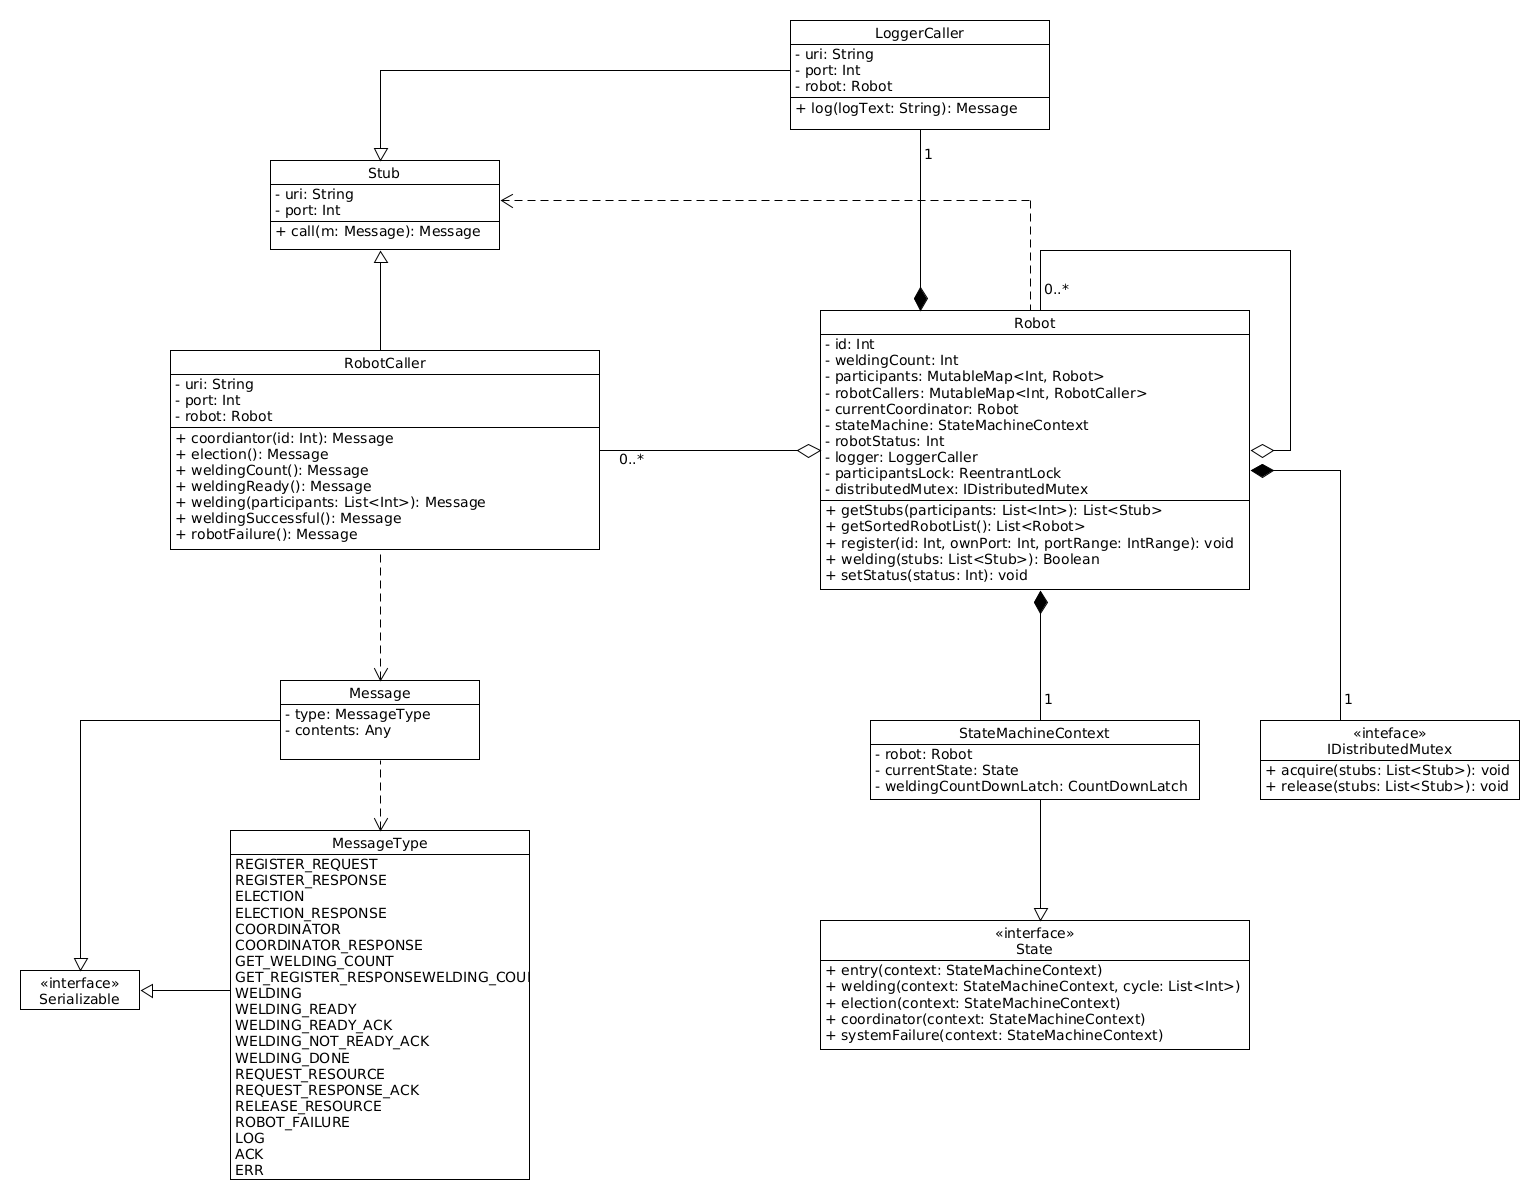
\includegraphics[width=\textwidth]{../diagrams/3_robot_klassendiagramm.png}
 \caption{Klassendiagramm Robot}
 \label{fig:class_robot}
\end{figure}

Im Klassendiagramm \ref{fig:class_robot} zu sehen ist die Implementierung der Robot-Klasse.
Wie vorher erwähnt sieht man hier die Bündelung der Funktionalitäten wie eine 
Instanz der FSM (StateMachineContext), den Robot- und LoggerCaller und den IDistributedMutex für
den verteilten gegenseitigen Ausschluss.

\clearpage

\subsection{Distributed Mutex}

\begin{figure}[h]
 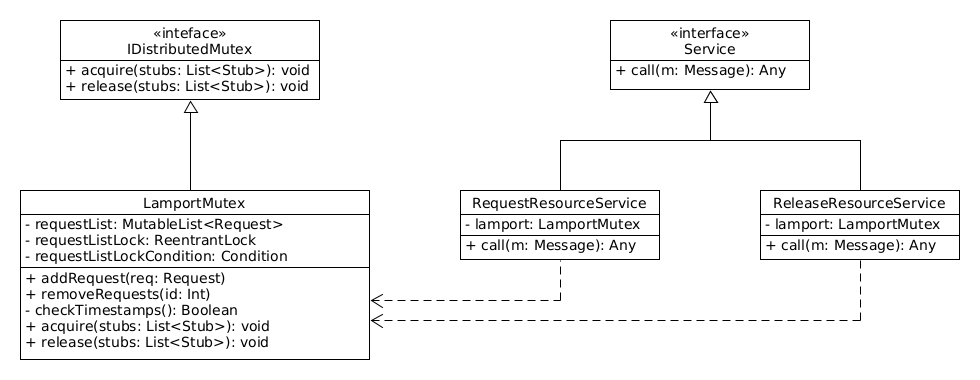
\includegraphics[width=\textwidth]{../diagrams/4_lamport_klassendiagramm.png}
 \caption{Klassendiagramm LamportMutex}
 \label{fig:class_lamport}
\end{figure}

In \ref{fig:class_lamport} zu sehen ist das Klassendiagramm des LamportMutex, der den Lamport-Algorithmus
implementiert. Damit die Austauschbarkeit des verwendeten Algorithmus (siehe \ref{table:reqmutexexchangable})
sichergestellt ist, wird das IDistributedMutex als Interface definiert und wie in \ref{fig:class_robot}
zu sehen im Robot mit der Implementierung des LamportMutex instanziiert. Die beiden Services RequestResourceService
und ReleaseResourceService sind Bestandteile der RPC-Architektur, über diese andere Roboter die Ressource
akquirieren (RequestResourceService) oder freigeben (ReleaseResourceService) können.

\clearpage

\subsection{FSM}

\begin{figure}[h]
 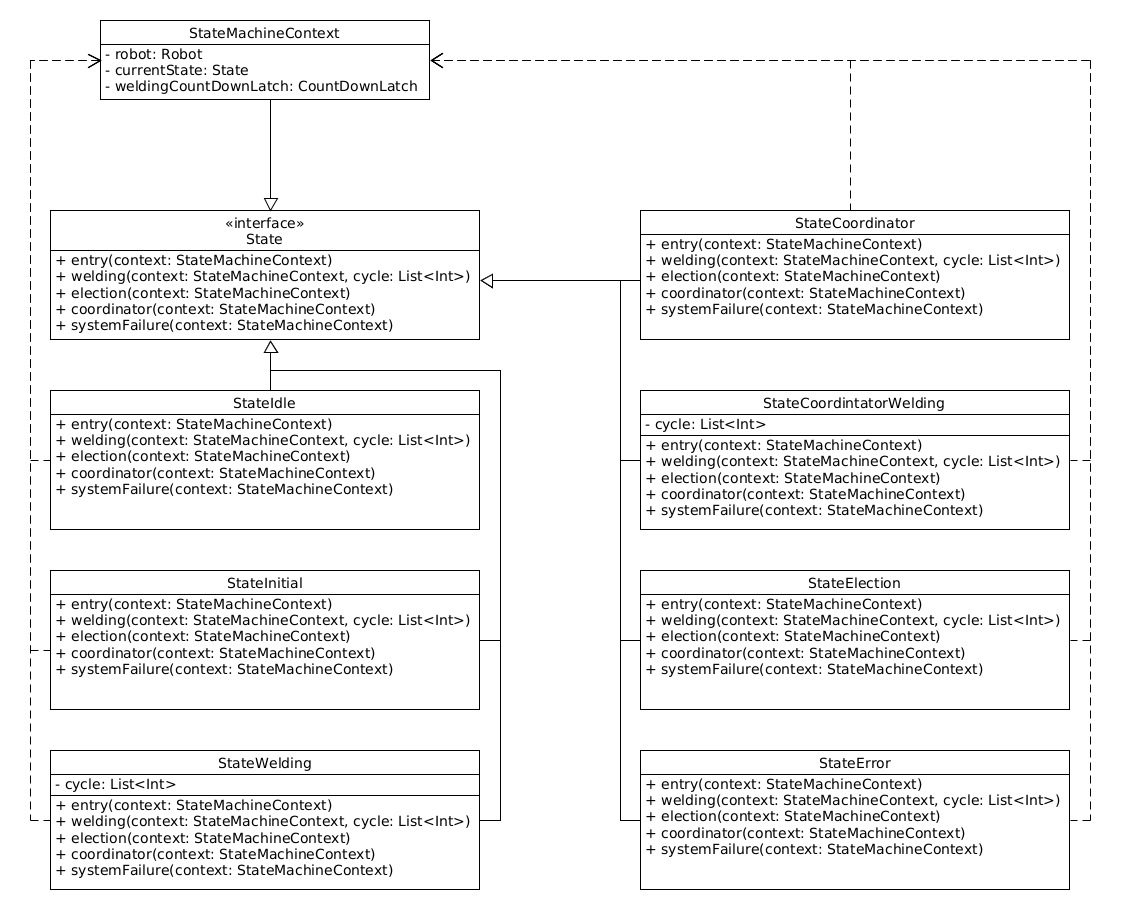
\includegraphics[width=\textwidth]{../diagrams/5_fsm_klassendiagramm.png}
 \caption{Klassendiagramm Statemachine}
 \label{fig:class_fsm}
\end{figure}

In Diagramm \ref{fig:class_fsm} ist das Klassendiagramm der FSM abgebildet. Für die Implementierung der FSM
wurde das State Pattern \citep{patterns} verwendet. Dieses ermöglicht eine übersichtliche und erweiterbare
Implementierung einer FSM, da jeder Zustand als Klasse implementiert ist und vom Interface \glqq State\grqq{}
(siehe \ref{fig:class_fsm}) erbt. Zum Hinzufügen von Zuständen muss eine neue Klasse implementiert werden, die 
von State erbt. Der StateMachineContext wird vom Roboter als Instanz gehalten und enthält zur Laufzeit immer
den aktuellen Zustand der FSM.

\subsection{Middleware}



\section{Laufzeitsicht}
